\section{Established components and the integration gap}
\label{sec:related}

\paragraph{Quantum optimization.}
QAOA alternates cost and mixer evolutions to produce a parameterized distribution over combinatorial states~\citep{farhi2014qaoa,zhou2020qaoa}; reviews document many encodings, mixers and optimizers~\citep{blekos2024review,sawaya2023mixers}. The alternating-operator formulation makes constraint-preserving mixers explicit~\citep{hadfield2019alternating}, while warm-start QAOA uses classical information in initialization~\citep{egger2021warm}. Quantum scheduling is likewise an existing research area rather than a novelty of this work~\citep{werner2026scheduling}. Recent Nature reviews map the reverse interface---AI for quantum computing and quantum-system characterization~\citep{artificialintelligence2025quantum,mehta2026representing}; our study instead audits quantum sampling inside an AI-governance allocation problem. We contribute neither a new circuit family nor a claim that deeper QAOA must perform better.

\paragraph{Organizations, uncertainty and governance.}
Chance-constrained programming formalizes tolerance to stochastic constraint failure~\citep{charnes1959chance}, while service-operations research studies staffing and capacity under uncertain demand~\citep{gans2003callcenters}. Human--AI work adds authority, complementarity and coordination questions~\citep{amershi2019humanai,seeber2020machines,fuegener2026complementarity}. Algorithmic work assignment can also affect perceived fairness and productivity~\citep{bai2022algorithmic}; consequently, our regional AI-use dispersion is labeled an \emph{exposure regularizer}, not a validated fairness metric~\citep{selbst2019fairness,mehrabi2021fairness}. NIST and ISO governance frameworks motivate documented risks, measurement and human accountability~\citep{nist2023airmf,iso42001,iso23894}, but do not certify our synthetic benchmark.

\paragraph{Selection, abstention and reproducibility.}
Selective classification and learning-to-defer ask a model to abstain or hand off under uncertainty~\citep{geifman2017selective,madras2018defer}; classical algorithm selection asks which solver fits an instance~\citep{rice1976algorithm,kotthoff2014algorithm}. Our frozen gate is related in spirit but materially weaker: because it uses QAOA optimum mass, it partitions evidence \emph{after} simulation and cannot save quantum computation. Null-inclusive locked evaluation follows reproducibility norms that emphasize complete protocols and inspectable artifacts~\citep{pineau2021reproducibility}.

\begin{figure}[t]
  \centering
  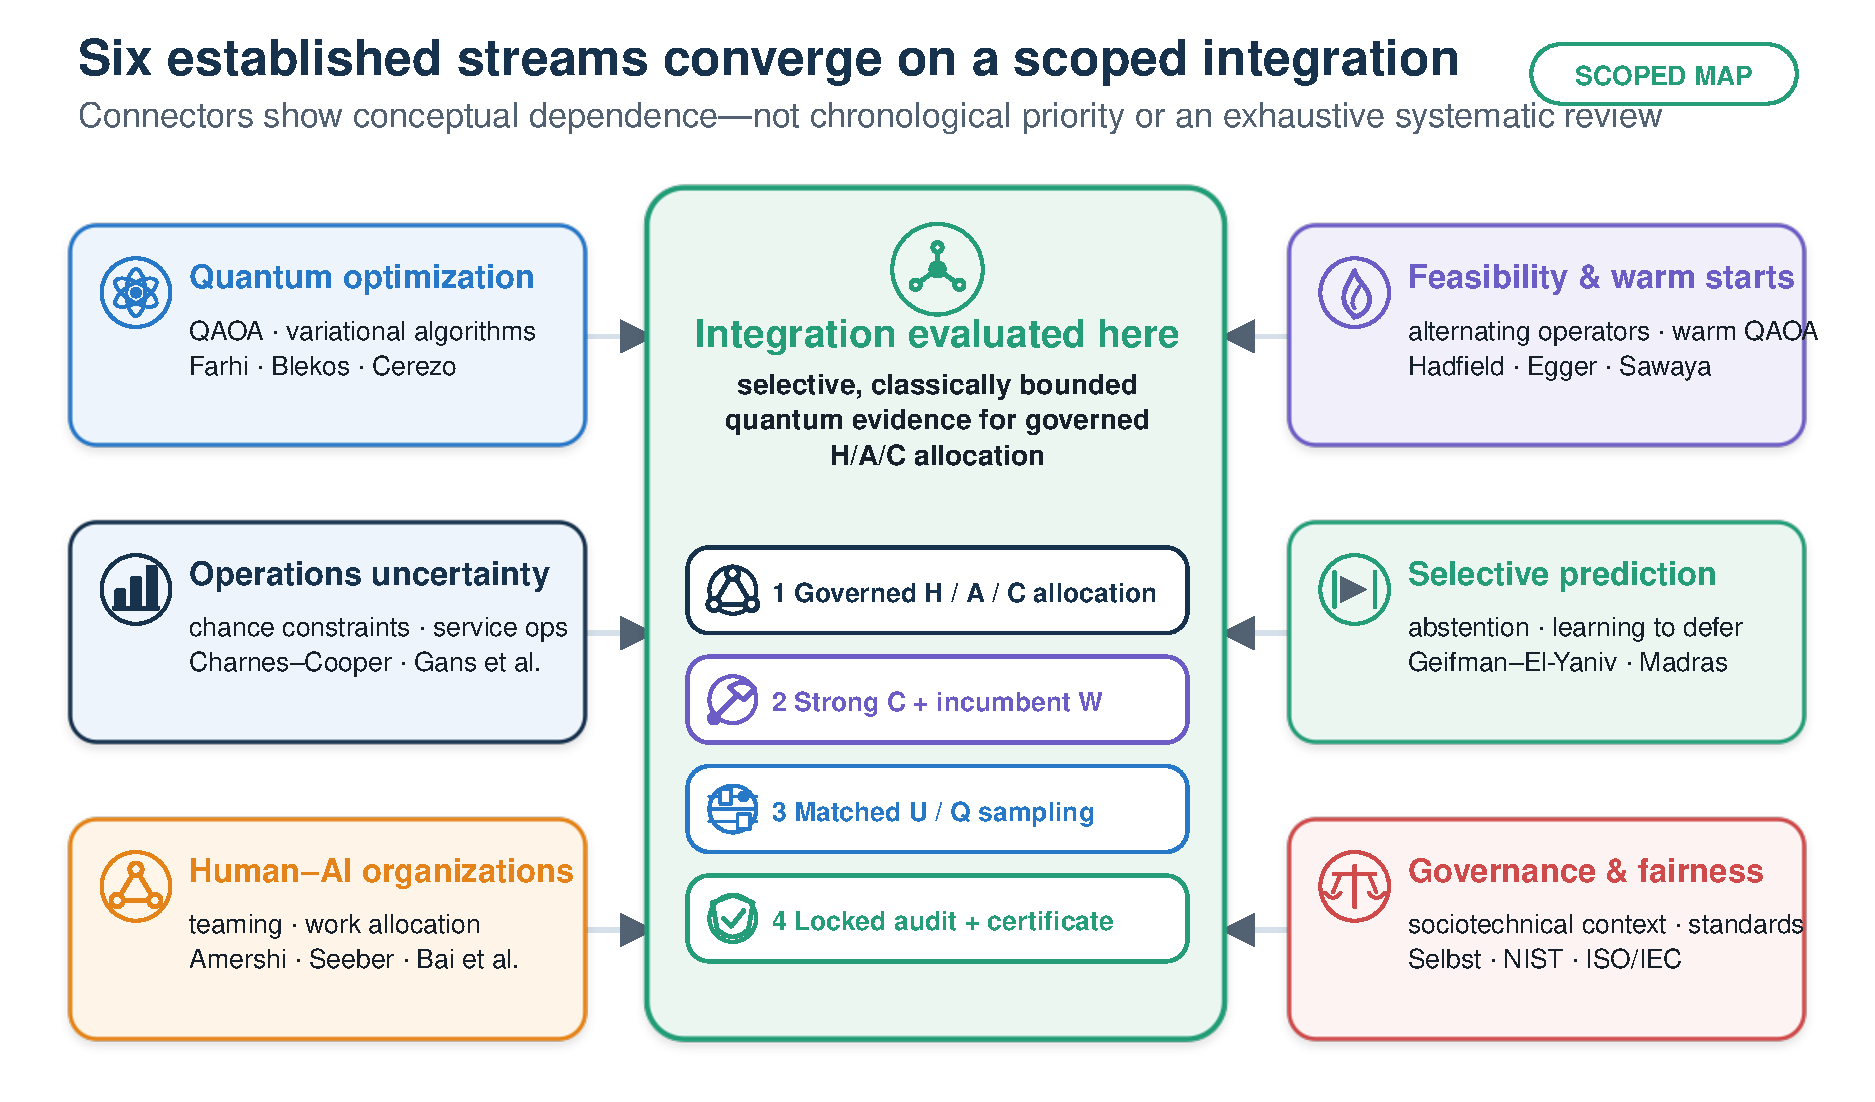
\includegraphics[width=\linewidth]{figs/fig4_literature_map.pdf}
  \caption{Scoped relationship map. Six established streams connect to the four-layer integration evaluated here: governed H/A/C allocation, strong classical structure and warm initialization, matched retained-set sampling, and locked classical certification. The short solid connectors encode conceptual dependence; the map is not a systematic-review flowchart or an exhaustive priority claim.}
  \label{fig:literature}
\end{figure}


\Cref{fig:literature} makes the novelty boundary visible. Each component is established. The gap addressed here is an auditable combination in which quantum sampling is conditioned on a governance-rich H/A/C evaluator, compared against strong classical structure, evaluated on held-out frozen instances, and bounded by a classical certificate. A systematic review could strengthen or refute this scoped integration claim; we do not infer ``first ever'' from the map.
